\section{Test-Framework}

\begin{frame}{Test-Framework - Allgemein}
Das Test-Framework wurde selbst implementiert. Es enthält diverse Funktionen zum automatisierten Überprüfen der Testfälle.

\par \medskip

\pause

Tests werden in korrekte und falsche Testfälle unterteilt.


\end{frame}

\begin{frame}[fragile]
	\frametitle{Test-Framework - Token-Coverage \& Testfälle}
	
Die Test-Suite umfasst eine Token-Coverage von 100\%. 

\pause

\par \medskip

Zusätzlich umfasst die Test-Suite insgesamt 21 gültige und 12 ungültige Testfälle.

\pause

\par \medskip

Ungültige Testfälle können in Syntaxfehler (Parser) und Typfehler (Typchecker) eingeteilt werden.
\end{frame}

\begin{frame}{Test-Framework - Testfälle}

Jedes Testfile liegt in einem Ordner (Correct bzw. Wrong) mit zugehöriger .java-Datei. 	

\pause 

\par \medskip

Ein Testfile besteht aus: 

\begin{itemize}
	\item Erwarteten Tokens \pause 
	\item Erwarteter abstrakter Syntax \pause 
	\item Erwarteter getypter abstrakter Syntax \pause
\end{itemize}

Zusätzlich zum eigentlichen Testfile enthält der Ordner ein ClassFile in Haskell, mit der zu erwartenden Struktur des erzeugten Classfiles.
\end{frame}

\begin{frame}[fragile]
\frametitle{Test-Framework - Beispiel Testfile}
\begin{center}
	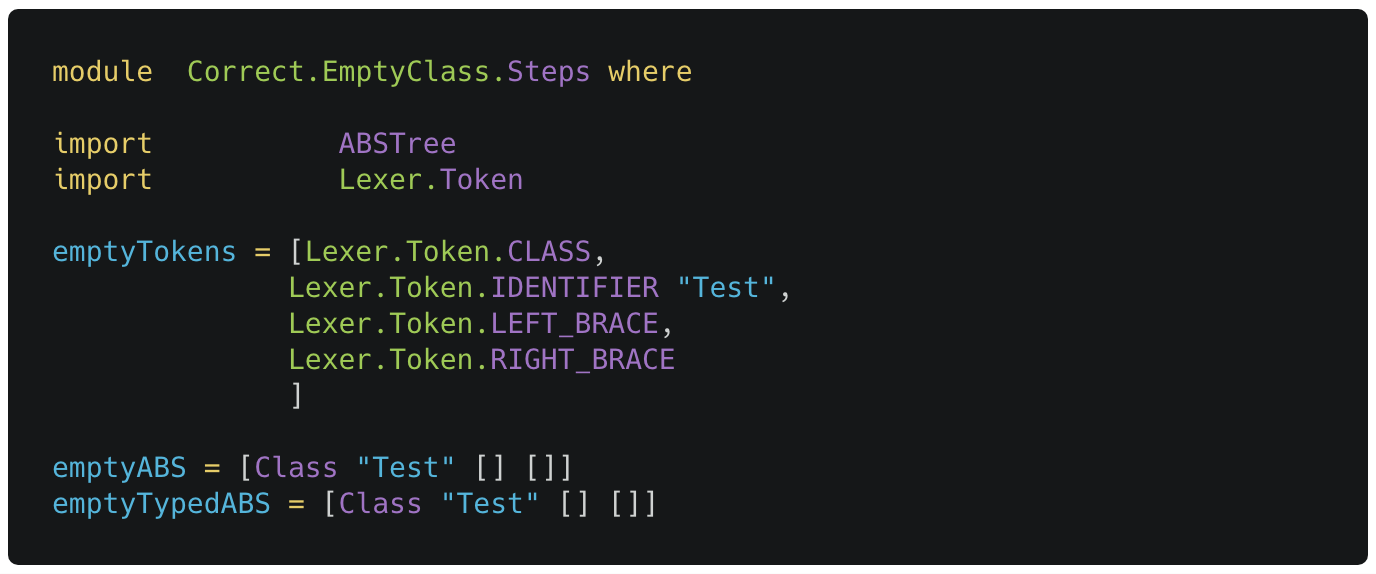
\includegraphics[width=1\textwidth]{images/test-framework/testfile}
\end{center}	
\end{frame}

\begin{frame}{Test-Framework - Beispielprogramme}
Die Testsuite enthält neben den Testfällen auch eine Reihe von (realistischeren) Anwendungsprogrammen. Diese wurden mit 'normalen' Javaprogrammen getestet und werden korrekt compiliert.
\pause

\begin{itemize}
	\item Multiplikation \pause 
	\item Gaußsumme (kleiner Gauß) \pause
	\item Fakultät \pause
	\item Fibonacci \pause
	\item Potenz $a^b$ \pause 
	\item $\lfloor \sqrt{x} \rfloor$ \pause
	\item Primzahltest \& nächste Primzahl ermitteln
\end{itemize}	
\end{frame}

\begin{frame}{Test-Framework: Demo}

	\begin{center}
		\huge{Demo}
	\end{center}
\end{frame}
